\documentclass[10pt]{beamer}
\usetheme[
%%% options passed to the outer theme
%    progressstyle=movCircCnt,   %either fixedCircCnt, movCircCnt, or corner
%    rotationcw,          % change the rotation direction from counter-clockwise to clockwise
%    shownavsym          % show the navigation symbols
  ]{AAUsimple}

% If you want to change the colors of the various elements in the theme, edit and uncomment the following lines
% Change the bar and sidebar colors:
%\setbeamercolor{AAUsimple}{fg=red!20,bg=red}
%\setbeamercolor{sidebar}{bg=red!20}
% Change the color of the structural elements:
%\setbeamercolor{structure}{fg=red}
% Change the frame title text color:
%\setbeamercolor{frametitle}{fg=blue}
% Change the normal text color background:
%\setbeamercolor{normal text}{fg=black,bg=gray!10}
% ... and you can of course change a lot more - see the beamer user manual.

\usepackage[utf8]{inputenc}
\usepackage[english]{babel}
\usepackage[T1]{fontenc}

\usepackage{pgf}
\usepackage{tikz}
\usepackage{marvosym}
\usetikzlibrary{positioning}
\usetikzlibrary{shapes}
\usetikzlibrary{arrows.meta}
\usetikzlibrary{arrows,automata}

\usepackage{graphicx}
\graphicspath{{/graphics/}}
\usepackage{tikzscale}


% Or whatever. Note that the encoding and the font should match. If T1
% does not look nice, try deleting the line with the fontenc.
\usepackage{helvet}
\usepackage{comment}

% colored hyperlinks
\newcommand{\chref}[2]{%
  \href{#1}{{\usebeamercolor[bg]{AAUsimple}#2}}%
}

\title{Smart Meter Security Analysis}

%\subtitle{Any suggestions for subtitle?}  % could also be a conference name

\date{\today}

\author{
  Bruno Thalmann\\
  Stefan Marstrand Getreuer Micheelsen\\
  Mikkel Sandø Larsen\\
  Mikael Elkiær Christensen
}

% - Give the names in the same order as they appear in the paper.
% - Use the \inst{?} command only if the authors have different
%   affiliation. See the beamer manual for an example

\institute[
%  {\includegraphics[scale=0.2]{aau_segl}}\\ %insert a company, department or university logo
  Dept.\ of Computer Science\\
  Aalborg University\\
  Denmark
] % optional - is placed in the bottom of the sidebar on every slide
{% is placed on the title page
  Department of Computer Science\\
  Aalborg University\\
  Denmark

  %there must be an empty line above this line - otherwise some unwanted space is added between the university and the country (I do not know why;( )
}

% specify a logo on the titlepage (you can specify additional logos an include them in
% institute command below
\pgfdeclareimage[height=1.5cm]{titlepagelogo}{AAUgraphics/aau_logo_new} % placed on the title page
%\pgfdeclareimage[height=1.5cm]{titlepagelogo2}{AAUgraphics/aau_logo_new} % placed on the title page
\titlegraphic{% is placed on the bottom of the title page
  \pgfuseimage{titlepagelogo}
%  \hspace{1cm}\pgfuseimage{titlepagelogo2}
}

\begin{document}
% the titlepage
{\aauwavesbg%
\begin{frame}[plain,noframenumbering] % the plain option removes the header from the title page
  \titlepage
\end{frame}}
%%%%%%%%%%%%%%%%

% CONTENT


\section*{Attacks}
\subsection*{Attacks in the context model}
\begin{frame}{Attacks in the context model}

\resizebox{!}{0.6\textwidth}
{
\tikzstyle{man}=[font={\Gentsroom}, scale=5]
\tikzstyle{woman}=[font={\Ladiesroom}, scale=5]

\begin{tikzpicture}[every node/.style={inner sep=0,outer sep=0}, arrows={[round]}]

\draw (-5.5,6) rectangle (2,-0.5);
\node at (-1,5.5) {Household};

\draw  (-6.5,7) [fill=white] rectangle (-4,5.5) node[pos=.5,align=center] {Home\\Production};
\draw  (-5,1.5) [fill=white] rectangle (-3.5,0) node[pos=.5,align=center] {Smart\\Meter};
\draw  (-3,4.5) [fill=white] rectangle (-1,3) node[pos=.5,align=center] {Smart\\Appliance};
\draw  (-0.5,2) [fill=white] rectangle (0.5,1) node[pos=.5,align=center] {Client};
\draw  (-9,2.5) [fill=white] rectangle (-6.5,1) node[pos=.5,align=center] {Data Hub};

\node[man] (consumer) at (1,1) {};
\node [below=0.2 of consumer] {Consumer};

\node[man] (burglar) at (-6.5,0) {};
\node [below=0.2 of burglar] {Burglar};

\node[man] (external) at (3.5,5) {};
\node [below=0.2 of external] {External};

\node[man] (power) at (-7.5,6.5) {};
\node [below=0.2 of power,align=center] {Electrical\\Company};

\node[man] (distribution) at (-7.5,4) {};
\node [below=0.2 of distribution] {Distribution};

\node[woman] (partner) at (1,4) {};
\node [below=0.2 of partner] {Partner};

\node[man] (neighbor) at (3.5,0.5) {};
\node [below=0.2 of neighbor] {Neighbor};

\draw[dashed] (-4.5,5.5) -- (-4.5,1.5);
\draw[dashed] (-6.5,1.5) -- (-6,1.5) -- (-6,1) -- (-5,1);
\draw[dashed] (-3.5,1) -- (-2.5,1) -- (-2.5,1.5) -- (-0.5,1.5);
\draw[dashed] (-2.5,3) -- (-2.5,2.25) -- (-4,2.25) -- (-4,1.5);

\draw[ultra thick, red, -{Stealth[scale=1.2]}, bend right=90] (power) to[out=-10,in=190] (consumer);
\draw[ultra thick, red, -{Stealth[scale=1.2]}, bend right] (consumer) to[out=-10,in=190] (power);

\draw[ultra thick, red, -{Stealth[scale=1.2]}] (neighbor) -- (consumer);
\draw[ultra thick, red, -{Stealth[scale=1.2]}] (partner) -- (consumer);
\draw[ultra thick, red, -{Stealth[scale=1.2]}] (burglar) -- (consumer);

\draw[ultra thick, red, -{Stealth[scale=1.2]}] (external) -- (consumer);


\end{tikzpicture}
}
\end{frame}

\begin{frame}{Consumer $\iff$ Electrical Company}

\resizebox{!}{0.6\textwidth}
{
\tikzstyle{man}=[font={\Gentsroom}, scale=5]
\tikzstyle{woman}=[font={\Ladiesroom}, scale=5]

\begin{tikzpicture}[every node/.style={inner sep=0,outer sep=0}, arrows={[round]}]

\draw (-5.5,6) rectangle (2,-0.5);
\node at (-1,5.5) {Household};

\draw  (-6.5,7) [fill=white] rectangle (-4,5.5) node[pos=.5,align=center] {Home\\Production};
\draw  (-5,1.5) [fill=white] rectangle (-3.5,0) node[pos=.5,align=center] {Smart\\Meter};
\draw  (-3,4.5) [fill=white] rectangle (-1,3) node[pos=.5,align=center] {Smart\\Appliance};
\draw  (-0.5,2) [fill=white] rectangle (0.5,1) node[pos=.5,align=center] {Client};
\draw  (-9,2.5) [fill=white] rectangle (-6.5,1) node[pos=.5,align=center] {Data Hub};

\node[man] (consumer) at (1,1) {};
\node [below=0.2 of consumer] {Consumer};

\node[man] (burglar) at (-6.5,0) {};
\node [below=0.2 of burglar] {Burglar};

\node[man] (external) at (3.5,5) {};
\node [below=0.2 of external] {External};

\node[man] (power) at (-7.5,6.5) {};
\node [below=0.2 of power,align=center] {Electrical\\Company};

\node[man] (distribution) at (-7.5,4) {};
\node [below=0.2 of distribution] {Distribution};

\node[woman] (partner) at (1,4) {};
\node [below=0.2 of partner] {Partner};

\node[man] (neighbor) at (3.5,0.5) {};
\node [below=0.2 of neighbor] {Neighbor};

\draw[dashed] (-4.5,5.5) -- (-4.5,1.5);
\draw[dashed] (-6.5,1.5) -- (-6,1.5) -- (-6,1) -- (-5,1);
\draw[dashed] (-3.5,1) -- (-2.5,1) -- (-2.5,1.5) -- (-0.5,1.5);
\draw[dashed] (-2.5,3) -- (-2.5,2.25) -- (-4,2.25) -- (-4,1.5);

\draw[ultra thick, red, -{Stealth[scale=1.2]}, bend right=90] (power) to[out=-10,in=190] (consumer);
\draw[ultra thick, red, -{Stealth[scale=1.2]}, bend right] (consumer) to[out=-10,in=190] (power);


\end{tikzpicture}
}
\end{frame}

\begin{frame}{Consumer $\implies$ Electrical Company}
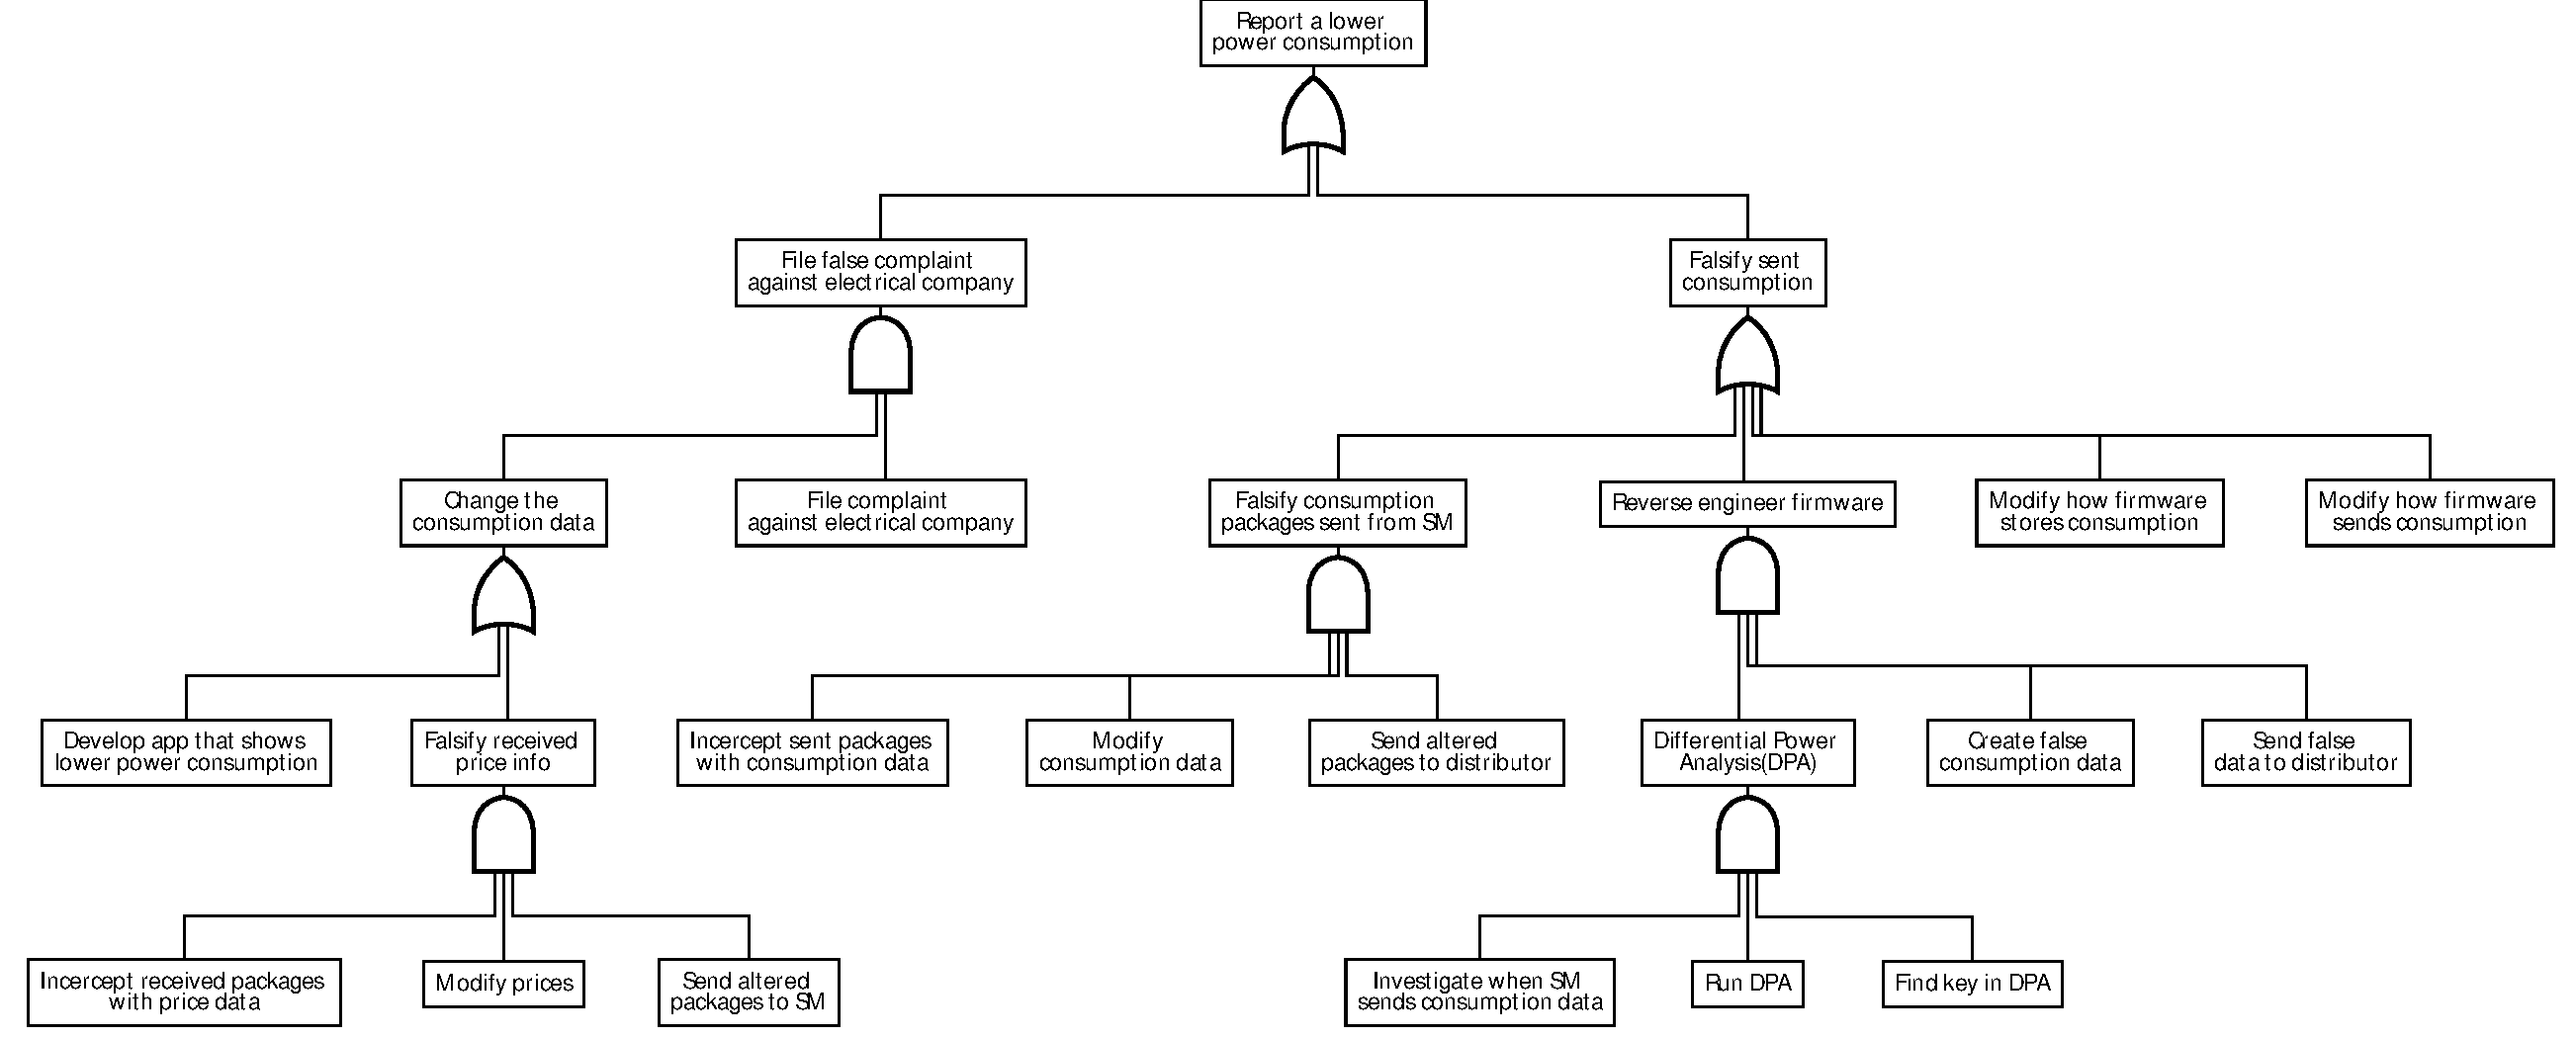
\includegraphics[width=1\textwidth]{graphics/consumer_orig.pdf}

\end{frame}

\begin{frame}{Consumer $\implies$ Electrical Company}
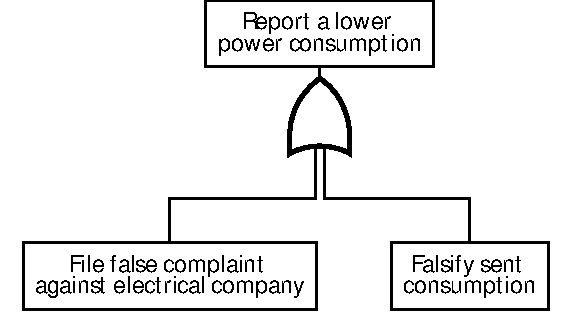
\includegraphics[width=1\textwidth]{graphics/consumer.pdf}

\end{frame}

\begin{frame}{Consumer $\impliedby$ Electrical Company}
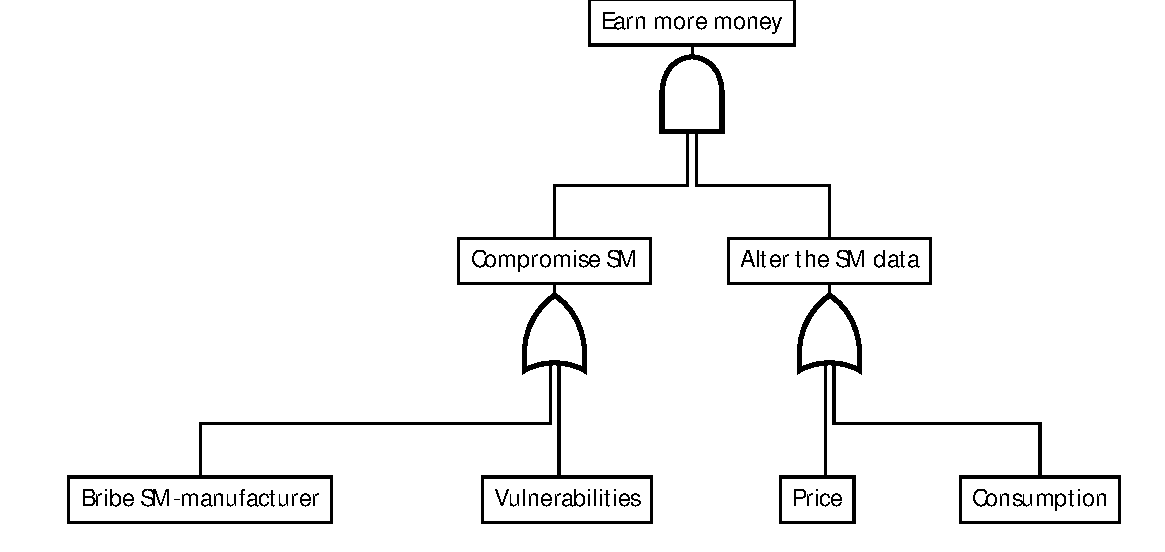
\includegraphics[width=\textwidth]{graphics/electrical_company_vs_consumer.pdf}

\end{frame}

\subsection*{Attacks against the consumer}
\begin{frame}{Attacks against the consumer}

\resizebox{!}{0.6\textwidth}
{
\tikzstyle{man}=[font={\Gentsroom}, scale=5]
\tikzstyle{woman}=[font={\Ladiesroom}, scale=5]

\begin{tikzpicture}[every node/.style={inner sep=0,outer sep=0}, arrows={[round]}]

\draw (-5.5,6) rectangle (2,-0.5);
\node at (-1,5.5) {Household};

\draw  (-6.5,7) [fill=white] rectangle (-4,5.5) node[pos=.5,align=center] {Home\\Production};
\draw  (-5,1.5) [fill=white] rectangle (-3.5,0) node[pos=.5,align=center] {Smart\\Meter};
\draw  (-3,4.5) [fill=white] rectangle (-1,3) node[pos=.5,align=center] {Smart\\Appliance};
\draw  (-0.5,2) [fill=white] rectangle (0.5,1) node[pos=.5,align=center] {Client};
\draw  (-9,2.5) [fill=white] rectangle (-6.5,1) node[pos=.5,align=center] {Data Hub};

\node[man] (consumer) at (1,1) {};
\node [below=0.2 of consumer] {Consumer};

\node[man] (burglar) at (-6.5,0) {};
\node [below=0.2 of burglar] {Burglar};

\node[man] (external) at (3.5,5) {};
\node [below=0.2 of external] {External};

\node[man] (power) at (-7.5,6.5) {};
\node [below=0.2 of power,align=center] {Electrical\\Company};

\node[man] (distribution) at (-7.5,4) {};
\node [below=0.2 of distribution] {Distribution};

\node[woman] (partner) at (1,4) {};
\node [below=0.2 of partner] {Partner};

\node[man] (neighbor) at (3.5,0.5) {};
\node [below=0.2 of neighbor] {Neighbor};

\draw[dashed] (-4.5,5.5) -- (-4.5,1.5);
\draw[dashed] (-6.5,1.5) -- (-6,1.5) -- (-6,1) -- (-5,1);
\draw[dashed] (-3.5,1) -- (-2.5,1) -- (-2.5,1.5) -- (-0.5,1.5);
\draw[dashed] (-2.5,3) -- (-2.5,2.25) -- (-4,2.25) -- (-4,1.5);


\draw<1>[ultra thick, red, -{Stealth[scale=1.2]}] (neighbor) -- (consumer);
\draw<1>[ultra thick, red, -{Stealth[scale=1.2]}] (partner) -- (consumer);
\draw<1>[ultra thick, red, -{Stealth[scale=1.2]}] (burglar) -- (consumer);

\draw<2>[ultra thick, red, -{Stealth[scale=1.2]}] (external) -- (consumer);


\end{tikzpicture}
}
\end{frame}

\begin{frame}{Attacks from the vicinity}
  Actors attacking the consumer have similar attack structure
\center
  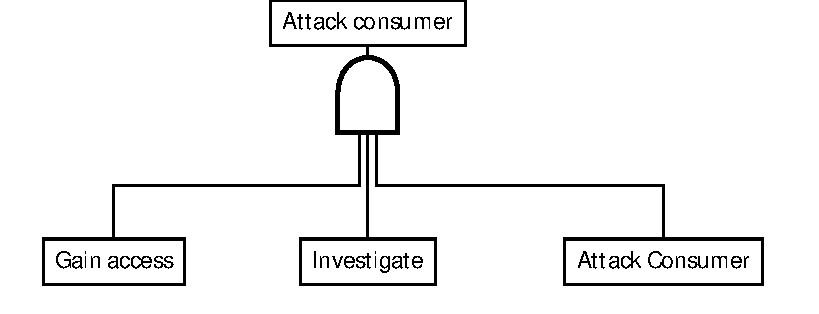
\includegraphics[width=0.7\textwidth]{graphics/common_attack.pdf}
\end{frame}

\begin{frame}{Gain access}
  \begin{block}{Accessing devices}
    \begin{itemize}
      \item Compromise Smart Meter
      \item Compromise Client
      \item Install ECM
    \end{itemize}
  \end{block}

  \begin{block}{Obtaining data }
    \begin{itemize}
      \item Buy power consumption data
      \item Obtain power consumption data through app or appliance
    \end{itemize}
  \end{block}
\end{frame}

\begin{frame}{Investigate}

\begin{tabular}{l l}

  
\includegraphics[width=0.4\textwidth]{graphics/hus.jpg}
&
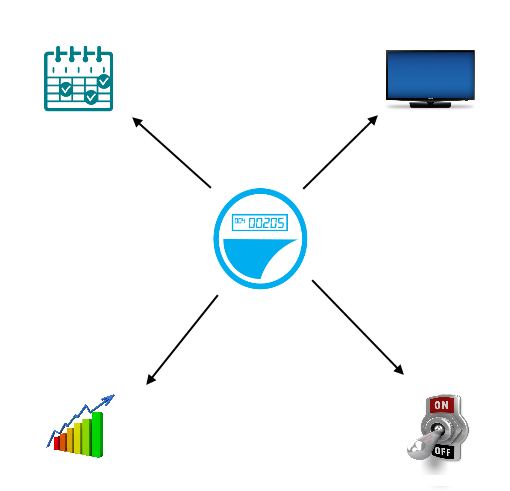
\includegraphics[width=0.4\textwidth]{graphics/smartmeterdata.png}
\end{tabular}

\end{frame}

\begin{frame}{Attack Consumer}
  \begin{columns}[T]
    \begin{column}{0.5\textwidth}
    \begin{block}{Direct attacks}
      Objective:
      \begin{itemize}
        \item Break in
        \item Remove annoyances
        \item Get revenge
      \end{itemize}
      Means:
      \begin{itemize}
        \item Control devices
        \item Change device schedules
      \end{itemize}
    \end{block}
\end{column}
\begin{column}{0.5\textwidth}
  \begin{block}{Indirect attacks}
    \begin{itemize}
      \item Create consumer profile
      \item Sell data
      \item Turn off power
    \end{itemize}
  \end{block}
\end{column}
\end{columns}
\end{frame}


% the final page
{\aauwavesbg
\begin{frame}[plain,noframenumbering]
  \finalpage{Thank you for your time}
\end{frame}}

\end{document}
